% Original book diagram: fig:book_roadmap_autonomy
% Book source: sections/back/conclusions.tex
% Original diagram authorship retained. Visual design: Ziad Mosalam.
\documentclass[11pt,border=8pt]{standalone}
\usepackage{amsmath,amssymb,graphicx,tikz}
\usetikzlibrary{arrows.meta,automata,positioning,calc,shapes.geometric,fit,backgrounds,patterns}
\newcommand{\vect}[1]{\mathbf{#1}}
\newcommand{\mat}[1]{\mathbf{#1}}
\newcommand{\Normal}{\mathcal{N}}
\newcommand{\prob}{p}
\newcommand{\E}{\mathbb{E}}
\newcommand{\Var}{\mathrm{Var}}
\newcommand{\Cov}{\mathrm{Cov}}
\newcommand{\CovP}{\mathbf{P}}
\newcommand{\Prob}{\mathbb{P}}
\setlength{\textwidth}{6.5in}
% Shared visual vocabulary for the book's original diagrams.
% Figures opt in explicitly, so unrelated text and existing additions are unchanged.
\definecolor{BookBlue}{HTML}{003262}
\definecolor{BookGold}{HTML}{B17A00}
\definecolor{BookTeal}{HTML}{247C86}
\definecolor{BookInk}{HTML}{30363B}
\definecolor{BookLight}{HTML}{E9EFF5}
\tikzset{
  book figure/.style={font=\small\rmfamily, color=BookBlue, text=BookInk,
    line width=0.8pt, >=Latex},
  book axis/.style={->, draw=BookInk, line width=0.6pt},
  book link/.style={->, draw=BookBlue, line width=0.8pt},
  book observation/.style={draw=BookGold, fill=BookGold!8},
  book state/.style={draw=BookBlue, fill=BookLight},
  book note/.style={font=\footnotesize\rmfamily, text=BookInk}
}

\begin{document}
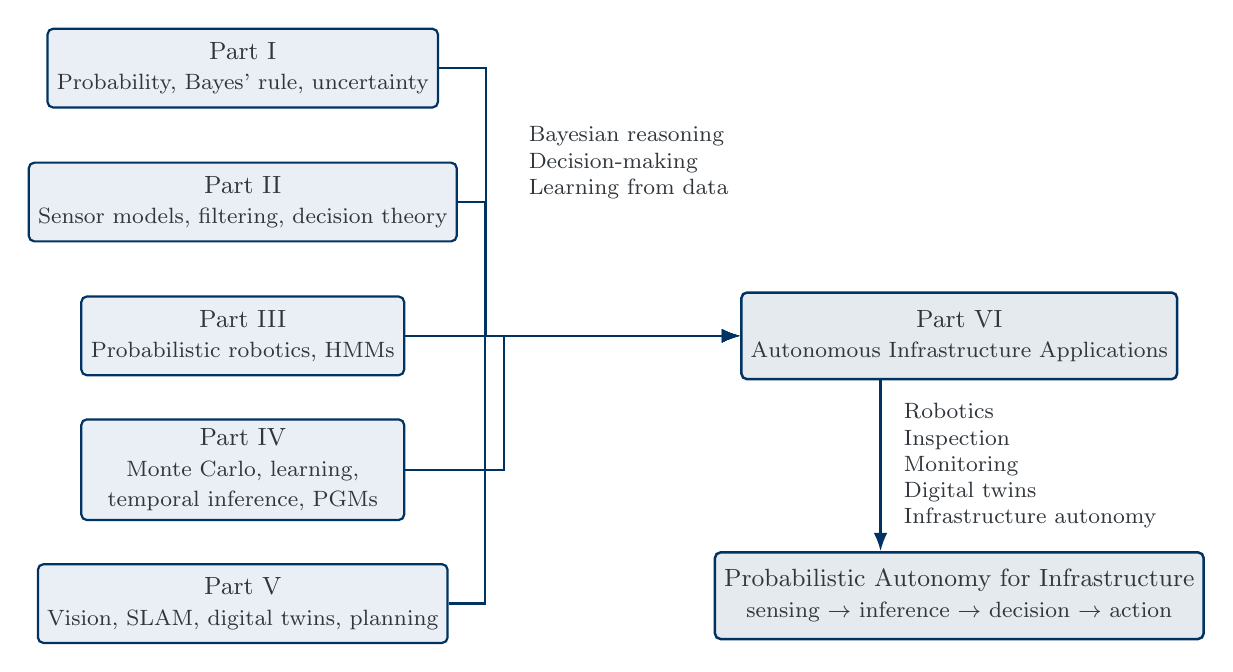
\begin{tikzpicture}[book figure,
>=Latex,
every node/.style={font=\small, align=center},
part/.style={
rectangle,
rounded corners=2pt,
draw,
minimum width=4.1cm,
minimum height=1.0cm,
line width=0.8pt,
fill=BookLight
},
core/.style={
rectangle,
rounded corners=2pt,
draw,
minimum width=4.4cm,
minimum height=1.1cm,
line width=0.9pt,
fill=BookBlue!10
},
arrow/.style={->, draw=BookBlue, line width=0.8pt}
]

% Left column
\node[part] (p1) at (0,7.5) {Part I\\{\footnotesize Probability, Bayes' rule, uncertainty}};
\node[part] (p2) at (0,5.8) {Part II\\{\footnotesize Sensor models, filtering, decision theory}};
\node[part] (p3) at (0,4.1) {Part III\\{\footnotesize Probabilistic robotics, HMMs}};
\node[part] (p4) at (0,2.4) {Part IV\\{\footnotesize Monte Carlo, learning,}\\{\footnotesize temporal inference, PGMs}};
\node[part] (p5) at (0,0.7) {Part V\\{\footnotesize Vision, SLAM, digital twins, planning}};

% Right application block
\node[core] (p6) at (9.1,4.1) {Part VI\\{\footnotesize Autonomous Infrastructure Applications}};

% Central synthesis node
\node[core] (core) at (9.1,0.8) {Probabilistic Autonomy for Infrastructure\\{\footnotesize sensing $\rightarrow$ inference $\rightarrow$ decision $\rightarrow$ action}};

% Arrows from parts to Part VI
\draw[arrow] (p1.east) -- ++(0.6,0) |- (p6.west);
\draw[arrow] (p2.east) -- ++(0.345,0) |- (p6.west);
\draw[arrow] (p3.east) -- ++(0.6,0) -- (p6.west);
\draw[arrow] (p4.east) -- ++(1.25,0) |- (p6.west);
\draw[arrow] (p5.east) -- ++(0.46,0) |- (p6.west);

% Arrow from Part VI to final synthesis
\draw[arrow] (p6.south) ++(-1.0,0) -- ([xshift=-1cm]core.north);

% Optional side notes
\node[font=\footnotesize, align=left] at (4.9,6.3)
{Bayesian reasoning\\Decision-making\\Learning from data};

\node[font=\footnotesize, align=left] at (10.0,2.45)
{Robotics\\Inspection\\Monitoring\\Digital twins\\Infrastructure autonomy};

\end{tikzpicture}
\end{document}
